In questa sezione verranno riportati in maniera schematica i valori effettivi riscontrati dalla misurazione delle metriche di processo e di prodotto in seguito alle operazioni di verifica della documentazione e del codice precedenti ad ogni revisione del progetto.
\subsection{Revisione dei Requisiti}
\subsubsection{Metriche processi}
\begin{table}[H]
\taburowcolors[2] 2{tableLineOne .. tableLineTwo}
\tabulinesep = 15pt
\everyrow{\tabucline[.4mm  white]{}}
\begin{tabu} to \textwidth { X[c,2] X[c,1] X[c,1] X[c,4] }
    \tableHeaderStyle
    ID & Valore & Esito & Commento \\
    \textbf{M[PROC][0001]} & 0 & Ottimo & Tutte le attività definite nel \PdPs sono state completate entro i tempi previsti. \\
    \textbf{M[PROC][0002]} & 185\euro{} & Ottimo & Come riportato nel consuntivo presente nel \PdPs è stato risparmiato un totale di 185\euro{} rispetto a quanto preventivato.  \\
    \textbf{M[PROC][0003]} & 0 & Ottimo &  Nel periodo precedente alla Revisione dei Requisiti non si sono presentati fattori di rischio non previsti dal \PdP. \\
    
\end{tabu}
\caption{Tabella resoconto dei valori misurati con le metriche di processo }
\end{table}

\newpage

\subsubsection{Metriche prodotto}
In questo periodo le metriche riguardanti il prodotto che sono state misurate riguardano l'indice di \citgl{Gulpease} per i documenti e la copertura del \citgl{framework} \citgl{Octalysis} basandoci sui requisiti individuati nel documento \AdR.

\subsubsection{M[PROD][D][0001]: Indice di Gulpease}

Il seguente grafico riporta, per tutti i documenti approvati ad eccezione del \G{}, i risultati delle misurazioni della metrica effettuate tramite lo strumento \citgl{Farfalla-Project}, come specificato nelle \NdP.

\begin{figure}[h!]
\begin{center}
  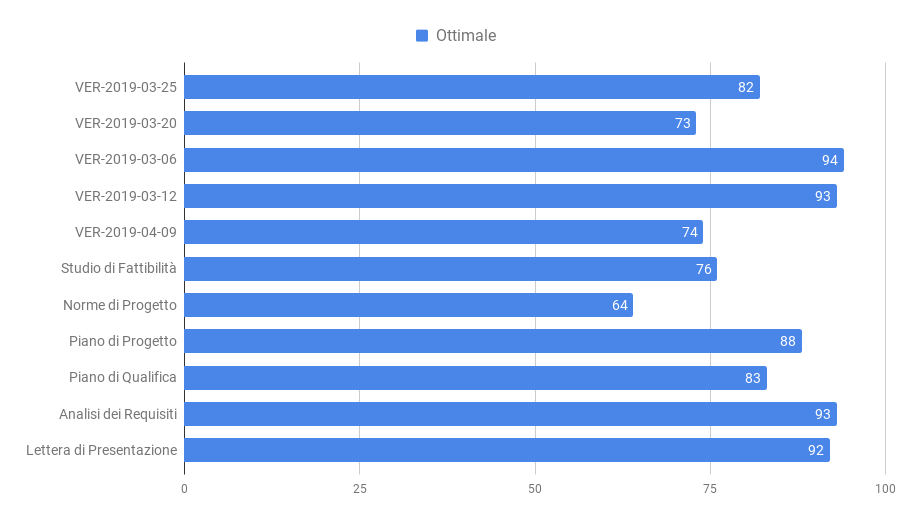
\includegraphics[scale=0.46]{immagini/GulpeaseG.png}
  \caption{Grafico valori indice Gulpease}
  \end{center}
\end{figure}


\subsubsection{M[PROD][S][0014]: Copertura del framework Octalysis}

\begin{table}[H]
\taburowcolors[2] 2{tableLineOne .. tableLineTwo}
\tabulinesep = 15pt
\everyrow{\tabucline[.4mm  white]{}}
\begin{tabu} to \textwidth { X[c,2] X[c,1] X[c,1] X[c,2] }
    \tableHeaderStyle
    Core Drive abbreviato & Quantità requisiti & Valore & Esito \\
    \textbf{Meaning} & 1 & 1 & Accettabile \\
    \textbf{Accomplishment} & 15 & 10 & Ottimo \\
    \textbf{Empowerment} & 1 & 1 & Accettabile  \\
    \textbf{Ownership} & 6 & 4 & Ottimo\\
    \textbf{Social Influence} & 5 & 3 &  Accettabile\\
    \textbf{Scarcity} & 0 & 0 & Ottimo\\
    \textbf{Unpredictability} & 2 & 1 & Ottimo\\
    \textbf{Avoidance} & 0 & 0 & Ottimo\\
\end{tabu}
\caption{Tabella resoconto copertura framework Octalysis}
\end{table}
\newpage
Il seguente grafico, ricavato tramite lo strumento online Octalysis-tool, riporta il codice di ogni requisito associato al relativo \citgl{Core Drive}. La dimensione di ogni area, identificata dal nome del Core Drive corrispondente, è proporzionale al valore raggiunto nella metrica sopra riportata.

\begin{figure}[h!]
\begin{center}
  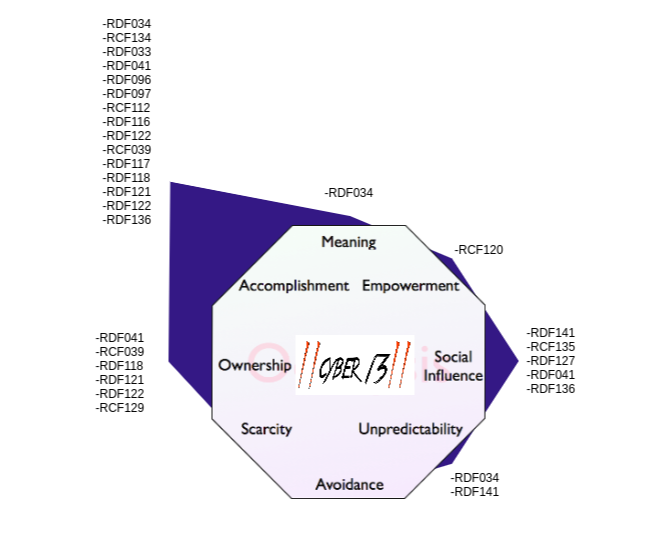
\includegraphics[scale=0.8]{immagini/Octalysys.png}
  \caption{Grafico copertura Core Drives Octalysys}
  \end{center}
\end{figure}


